% ______________________________________________________________________________
%
% DVG001 -- Introduktion till Linux och små nätverk
%                                     Projektarbete
% ~~~~~~~~~~~~~~~~~~~~~~~~~~~~~~~~~~~~~~~~~~~~~~~~~
% Author:   Jonas Sjöberg
%           tel12jsg@student.hig.se
%
% Date:     2016-06-07 -- 2016-06-13
%
% License:  Creative Commons Attribution 4.0 International (CC BY 4.0)
%           <http://creativecommons.org/licenses/by/4.0/legalcode>
%           See LICENSE.md for additional licensing information.
% ______________________________________________________________________________

\documentclass[11pt,a4paper]{article}

\usepackage[utf8]{inputenc}
\inputencoding{utf8}
\usepackage[swedish]{babel}
\usepackage[swedish]{isodate}
\usepackage[T1]{fontenc}

\usepackage{lmodern}
\usepackage{fullpage}

\usepackage{csquotes}               % Behövs av biblatex

\usepackage[natbib=true,
            style=ieee,
            backend=biber]{biblatex}
\addbibresource{tex/refs.bib}

\usepackage[binary-units=true]{siunitx}
\usepackage{float}
\usepackage{textcomp}
\usepackage{url}
\usepackage{graphicx}
%\usepackage{amssymb}
%\usepackage{amsmath}
\usepackage{amsfonts}
\usepackage{graphicx}
%\usepackage{microtype}

\usepackage[pdfusetitle,
            bookmarks=true,
            bookmarksnumbered=true,
            bookmarksopen=false,
            breaklinks=false,
            pdfborder={0 0 0},
            backref=false,
            colorlinks=false,
            hidelinks]{hyperref}

\newcommand{\screenshot}[4]{
\begin{figure}[H]
\centering
%\includegraphics[width=\linewidth]{#1}
\includegraphics[height=8.0cm]{#1}
\caption[#2]{#3}
\label{#4}
\end{figure}
}

\usepackage{minted}
\usemintedstyle{bw}

\usepackage{verbatim}
\usepackage{fancyvrb}
\usepackage{listings}

\newmintedfile[shellcode]{bash}{
%bgcolor=mintedbackground,
%fontfamily=tt,
breaklines=true,
fontsize=\footnotesize,
linenos=true,
numberblanklines=true,
numbersep=12pt,
numbersep=5pt,
%gobble= 0,
frame= lines,
%framerule= 0.4pt,
framesep=2mm,
funcnamehighlighting=true,
tabsize=4,
obeytabs=false,
mathescape=false
samepage=false,
showspaces=false,
showtabs=false,
texcl=false,
}

\newmintedfile[configfile]{linux-config}{
%bgcolor=mintedbackground,
%fontfamily=tt,
fontsize=\footnotesize,
linenos=true,
numberblanklines=true,
numbersep=12pt,
numbersep=5pt,
%gobble=0,
frame=lines,
%framerule=0.4pt,
framesep=2mm,
funcnamehighlighting=true,
tabsize=4,
obeytabs=false,
mathescape=false
samepage=false,
showspaces=false,
showtabs=false,
texcl=false,
}

\newmintedfile[markdownfile]{markdown}{
%bgcolor=mintedbackground,
%fontfamily=tt,
breaklines=true,
breakautoindent=true,
fontsize=\footnotesize,
linenos=true,
numberblanklines=true,
numbersep=12pt,
numbersep=5pt,
%gobble=0,
frame=lines,
%framerule=0.4pt,
framesep=2mm,
funcnamehighlighting=true,
tabsize=4,
obeytabs=false,
mathescape=false
samepage=false,
showspaces=false,
showtabs=false,
texcl=false,
}

\expandafter\def\csname PY@tok@err\endcsname{}
\expandafter\def\csname PYGdefault@tok@err\endcsname{\def\PYGdefault@bc##1{{\strut ##1}}}

\renewcommand\listingscaption{Programlistning}
\renewcommand\listoflistingscaption{Programlistningar}

\usepackage{booktabs}
\usepackage{longtable}

\usepackage{pdfpages}

\newcommand{\shellsource}[3]{
\begin{listing}[H]
\shellcode{#1}
\caption{#2}
\label{#3}
\end{listing}
}

\newcommand{\configsource}[3]{
\begin{listing}[H]
\configfile{#1}
\caption{#2}
\label{#3}
\end{listing}
}

\newcommand{\screenshot}[4]{
\begin{figure}[H]
\centering
\includegraphics[width=\linewidth]{#1}
%\includegraphics[height=8.0cm]{#1}
\caption[#2]{#3}
\label{#4}
\end{figure}
}


\title{\textsc{DVG001}                         \\
       Introduktion till Linux och små nätverk \\
       Projektarbete}

\author{                                 \\
  Jonas Sjöberg                          \\
  860224-xxxx                            \\
  Högskolan i Gävle                      \\
  \texttt{tel12jsg@student.hig.se}       \\
  \texttt{https://github.com/jonasjberg} \\
}

\date{}

\begin{document}
  \maketitle

  \begin{center}
    \begin{tabular}{l r} 
      Utförd:              & \isodate \printdate{2016-06-07} -- \printdate{2016-06-13} \\
      Kursansvarig lärare: & Anders Jackson                                            \\
                           & Anders Hermansson
    \end{tabular}
  \end{center}

  \begin{abstract}
    Projektarbete i kursen \emph{DVG001 -- Introduktion till Linux och små
    nätverk} som läses på distans via Högskolan i Gävle under vårterminen 2016.
    Under projektarbetet ska en server konfigureras för att göra vissa tjänster
    tillgängliga över \texttt{IPv6}.
    Projektet innehåller en stor mängd av de områden kursen har behandlat,
    särskilt konfigurering av webbserver och filserver, installation och
    konfigurering av brandvägg, upprättande av nätverk och hantering av en
    mängd protokoll och program.
  \end{abstract}

  \newpage
  %\hypersetup{linkcolor=black}
  \setcounter{tocdepth}{3}
  \tableofcontents

  \bigskip

  \listoffigures
  %\listoftables
  \listoflistings

  %\expandafter\def\csname PY@tok@err\endcsname{}

  \newpage
  % ______________________________________________________________________________
%
% DVG001 -- Introduktion till Linux och små nätverk
%                                     Projektarbete
% ~~~~~~~~~~~~~~~~~~~~~~~~~~~~~~~~~~~~~~~~~~~~~~~~~
% Author:   Jonas Sjöberg
%           tel12jsg@student.hig.se
%
% Date:     2016-06-07 -- 2016-06-13
%
% License:  Creative Commons Attribution 4.0 International (CC BY 4.0)
%           <http://creativecommons.org/licenses/by/4.0/legalcode>
%           See LICENSE.md for additional licensing information.
% ______________________________________________________________________________


\section{Inledning}
% Skriv en kort inledning här som beskriver kortfattat vad rapporten handlar
% om. Den skall vara orienterande om Bakgrund och Syfte.
% TODO: ..


% ______________________________________________________________________________
\subsection{Bakgrund}
% Beskriv lite mer ingående om bakgrunden till uppgiften, vad den handlar om.
Laborationen bygger vidare på de föregående laborationerna och behandlar vidare
praktisk användning av \texttt{IPv6} genom installation och konfiguration av
en server för direkt åtkomst genom olika protokoll över internet.

Den virtuella maskin som skapades tidigare under kursens gång används under
laborationen och kommer bland annat att få agera server och demonstrera vanligt
förekommande verktyg och program för nätverksadministration.

% ______________________________________________________________________________
\subsection{Syfte}
% Skriv lite mer ingående om syftet med uppgiften.
Syftet med laborationen är att vidare demonstrera och ge ytterligare tillfälle
till att öva praktisering av systemadministration, särskilt relaterat till
servrar och nätverk.

% ______________________________________________________________________________
\subsection{Arbetsmetod}
% Hur kommer ni att arbeta?  Detta är en lite längre text än den rent
% orienterande texten i Planering och genomförande ovan.

Nedan följer en preliminär redogörelse för den experimentuppställning som
användes under laborationen:

\begin{itemize}
  \item Laborationen utförs på en \texttt{ProBook-6545b} laptop som kör
        \texttt{Xubuntu 16.04} på kerneln \texttt{Linux 4.4.0-21}.  Under
        tidigare laborationer körde värdsystemet ett 32-bitars operativsystem.
        Innan denna laboration uppgraderades värdsystemets operativsystem och
        då till en 64-bitars version. Förändringen i arkitektur har ännu inte
        krävt några justeringar av den virtuella maskinen som upprättats för
        kursarbetet.

  \item Rapporten skrivs i \LaTeX\  som kompileras till pdf med \texttt{latexmk}.
        Detta sker på värdsystemet.

  \item Virtualisering sker med \texttt{Oracle VirtualBox} version
        \texttt{5.0.18\_Ubuntu r106667}.

  \item Utveckling av programkod och testkörning sker i gästsystemet som kör
        \texttt{Debian 7.3 (jessie)} på kerneln \texttt{Linux 3.16.0-4}.

  \item Både rapporten och eventuell kod skrivs med texteditorn \texttt{Vim}.

  \item För versionshantering av både rapporten och programkod används \texttt{Git}.
    \begin{itemize}
      \item Källkod till programmet och rapporten finns att hämta på:

            \url{https://github.com/jonasjberg/DVG001\_project}

      \item Hämta hem repon genom att exekvera följande från kommandoraden:
            
            \texttt{git clone git@github.com:jonasjberg/DVG001\_project.git}

    \end{itemize}
\end{itemize}



  % ______________________________________________________________________________
%
% DVG001 -- Introduktion till Linux och små nätverk
%                                     Projektarbete
% ~~~~~~~~~~~~~~~~~~~~~~~~~~~~~~~~~~~~~~~~~~~~~~~~~
% Author:   Jonas Sjöberg
%           tel12jsg@student.hig.se
%
% Date:     2016-06-07 -- 2016-06-13
%
% License:  Creative Commons Attribution 4.0 International (CC BY 4.0)
%           <http://creativecommons.org/licenses/by/4.0/legalcode>
%           See LICENSE.md for additional licensing information.
% ______________________________________________________________________________


\section{Skapande av IPv6-tunnel}
% ______________________________________________________________________________
\subsection{Registrering av tunnelservice}
% TODO: Skriv om registrering av konto för tunnel på https://www.tunnelbroker.net.
För tunnel-service valdes gratistjänsten ``Tunnel Broker'' som erbjuds av
Hurricane Electric.  Som ett första steg registrerades ett nytt konto. Sedan
skapades en tunnel genom Hurricane Electrics web-interface för inloggade
användare. Detta visas i Figur~\ref{fig:01}.

\screenshot{include/01_tunnelbroker_new-tunnel}
           {Skärmdump på skapande av en ny tunnel.}
           {Skärmdump på skapande av en ny IPv6-tunnel i Hurricane Electrics
            web-interface.}
           {fig:01}


\subsection{Statisk IP-adress för Debian-maskinen}
\subsubsection{Konfigurationsfilen \texttt{/etc/network/interfaces}}
För att ge Debian-maskinen en statisk IP-adress ändrades filen \texttt{/etc/network/interfaces}
för att få utseendet enligt Programlistning~\ref{listing:interfaces-static-ip}.

\configsource{include/conf_interfaces-static-ip}
            {Innehåll i konfigurationsfilen \texttt{/etc/network/interfaces}
 					   för statisk IP-adress.}
            {listing:interfaces-static-ip}


\subsubsection{Konfiguration av router}
I nätverkets routern reserveras en IP-adressen \texttt{192.168.1.112} till
Debian-maskinens MAC-adress.


\subsection{Konfiguration av tunneln}
Konfigurationen av tunneln sköts också genom att ändra i filen
\texttt{/etc/network/interfaces}, som får utseendet enligt
Programlistning~\ref{listing:interfaces-all}.

\configsource{include/conf_interfaces-all}
            {Fullständigt innehåll i konfigurationsfilen \texttt{/etc/network/interfaces}.}
            {listing:interfaces-all}


Raden \texttt{auto heipv6} gör att tunneln startas automatiskt.
Efter omstart visas den nya tunneln bland aktiva interface. Detta visas i  
Programlistning~\ref{listing:ifconfig}.

\shellsource{include/cmd_ifconfig}
            {Verifiering av ändringar i \texttt{/etc/network/interfaces}
             genom körning av \texttt{ifconfig}.}
            {listing:ifconfig}

% ______________________________________________________________________________
\subsection{Test av tunneln}
Anslutningen testas genom att köra kommandon enligt 
Programlistning~\ref{listing:ip_addr-route} och \ref{listing:ping6}.

\shellsource{include/cmd_ip_addr-route}
            {Kontroll av IPv6-tunnelns status.}
            {listing:ip_addr-route}

\shellsource{include/cmd_ping6}
            {Test av ICMP/ping till server över IPv6.}
            {listing:ping6}

Anslutningen verifieras också med hemsidorna \texttt{http://test-ipv6.com/}
och \texttt{http://ipv6-test.com/} enligt skärmdumpar i Figur~\ref{fig:02}
och Figur~\ref{fig:03}.
Anslutning till servern \texttt{http://rigel.hig.se} visas i
Figur~\ref{fig:04}.

\screenshot{include/02_ipv6test}
           {Skärmdump på test av anslutningar.}
           {Skärmdump på test av anslutningar till nätverket från med tjänsten
            på \texttt{http://ipv6-test.com/}.}
           {fig:02}

\screenshot{include/03_test-ipv6}
           {Skärmdump på test av anslutningar.}
           {Skärmdump på test av anslutningar till nätverket från med tjänsten
            på \texttt{http://test-ipv6.com/}.}
           {fig:03}

\screenshot{include/04_rigel-hig-se}
           {Skärmdump på test av anslutning.}
           {Skärmdump på test av IPv6 genom anslutning till
            \texttt{http://rigel.hig.se}.}
           {fig:04}


  % ______________________________________________________________________________
%
% DVG001 -- Introduktion till Linux och små nätverk
%                                     Projektarbete
% ~~~~~~~~~~~~~~~~~~~~~~~~~~~~~~~~~~~~~~~~~~~~~~~~~
% Author:   Jonas Sjöberg
%           tel12jsg@student.hig.se
%
% Date:     2016-06-07 -- 2016-06-13
%
% License:  Creative Commons Attribution 4.0 International (CC BY 4.0)
%           <http://creativecommons.org/licenses/by/4.0/legalcode>
%           See LICENSE.md for additional licensing information.
% ______________________________________________________________________________


% ______________________________________________________________________________
\section{Konfiguration av servern}
\subsection{Konfiguration av fjärråtkomst}
En del av projektets redovisning kräver att läraren ska kunna logga in på servern
med SSH genom att använda serverns IPv6-adress. Här förbereds inför detta.


% ______________________________________________________________________________
\subsection{Registrering av DNS-tjänst}
För att underlätta test och ge en mer lätthanterlig adress registrerades ett
konto hos \texttt{dynv6} \cite{ipv6:dynv6}, som erbjuder en gratis dynamisk
DNS-tjänst. Detta efter tips på kursens Blackboard-forum.

På så vis kan servern nås med en mer ``\emph{human-readable}'' adress,
som i det här fallet valdes att vara \texttt{http://jonasjberg.dynv6.net}.

För att testa adressen användes en IPv6-proxy \cite{ipv6:ipv6proxy}.
Resultatet av testet visas i Figur~\ref{fig:05}.

\screenshot{include/05_ipv6proxy}
           {Skärmdump på test av anslutning till \texttt{dynv6.net}-adressen.}
           {Skärmdump på test av anslutning till \texttt{dynv6.net}-adressen 
					  \texttt{http://jonasjberg.dynv6.net} genom en IPv6-proxy.}
           {fig:05}


% ______________________________________________________________________________
\subsubsection{Ny användare \texttt{higjxn}}
En ny användare som läraren kan använda vid inloggning skapas med kommandot
\texttt{adduser higjxn}.

Den nya användaren läggs till i grupperna \texttt{adm} och \texttt{sudo} för
att möjliggöra kontroll av serverns konfiguration och loggar. Detta görs med
kommandot \texttt{adduser}.


% ______________________________________________________________________________
\subsection{Test av fjärråtkomst}
Test av inloggning över SSH med användaren \texttt{higjxn} visas i
Programlistning~\ref{listing:ssh-higjxn}.

\shellsource{include/cmd_ssh-higjxn}
            {Test av SSH med användaren \texttt{higjxn}.}
            {listing:ssh-higjxn}

Ett andra test av åtkomst över SSH med hjälp av ett onlineverktyg på adressen
\url{http://www.infobyip.com/sshservertest.php} \cite{ipv6:sshservertest}
visas i Figur~\ref{fig:06}.

\screenshot{include/06_ssh-test}
           {Skärmdump på test av SSH-server.}
					 {Skärmdump på test av SSH-anslutning med hjälp av onlineverktyget 
				    \texttt{http://www.infobyip.com/sshservertest.php}.}
           {fig:06}


% ______________________________________________________________________________
\subsection{Servern som lokal IPv6-router}
Debian-servern kan konfigureras för att agera router åt övriga datorer i det
lokala nätverket. På så vis kan de också göra IPv6-anslutningar.

Till att börja med ändrades filen \texttt{/etc/sysctl.conf}. Den ändrade
raden visas i Programlistning~\ref{listing:sysctl}.

\configsource{include/conf_sysctl}
             {Utdrag ur konfigurationsfilen \texttt{/etc/sysctl.conf}.}
             {listing:sysctl}

  % ______________________________________________________________________________
%
% DVG001 -- Introduktion till Linux och små nätverk
%                                     Projektarbete
% ~~~~~~~~~~~~~~~~~~~~~~~~~~~~~~~~~~~~~~~~~~~~~~~~~
% Author:   Jonas Sjöberg
%           tel12jsg@student.hig.se
%
% Date:     2016-06-07 -- 2016-06-13
%
% License:  Creative Commons Attribution 4.0 International (CC BY 4.0)
%           <http://creativecommons.org/licenses/by/4.0/legalcode>
%           See LICENSE.md for additional licensing information.
% ______________________________________________________________________________


% ______________________________________________________________________________
\section{Servern som lokal IPv6-router}
Debian-servern kan konfigureras för att agera router åt övriga datorer i det
lokala nätverket. På så vis kan de också göra IPv6-anslutningar.

Till att börja med ändrades filen \texttt{/etc/sysctl.conf}. Den ändrade
raden visas i Programlistning~\ref{listing:sysctl}.

\configsource{include/conf_sysctl}
             {Utdrag ur konfigurationsfilen \texttt{/etc/sysctl.conf}.}
             {listing:sysctl}

\subsection{DMZ}
Det lokala nätverkets router ställs in att först skicka all trafik till
Debian-servern genom att \texttt{DMZ} aktiveras i routerns konfiguration genom
ett konfigurationsinterface som nås genom en webbläsare.
Detta visas i Figur~\ref{fig:dmz}.

\begin{figure}[H]
  \centering
  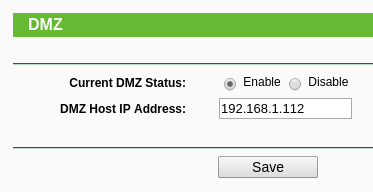
\includegraphics[width=0.5\linewidth]{include/dmz}
  \caption[Skärmdump på inställning av \texttt{dmz}]
          {Skärmdump på inställning av \texttt{dmz} i nätverkets router.}
  \label{fig:dmz}
\end{figure}


% ______________________________________________________________________________
\subsection{Konfigurationsfiler}
\subsubsection{\texttt{/etc/network/interfaces}}
Konfigurationsfilen \texttt{/etc/network/interfaces} har nu det slutgiltiga
utseendet i Programlistning~\ref{listing:interfaces-final}.

\configsource{include/conf_interfaces-final}
						 {Slutgiltigt innehåll i konfigurationsfilen
					    \texttt{/etc/network/interfaces}.}
             {listing:interfaces-final}


\subsubsection{\texttt{/etc/radvd.conf}}
Konfigurationsfilen \texttt{/etc/radvd.conf} får utseendet i
Programlistning~\ref{listing:radvd} för att Debian-servern ska fungera som
lokal IPv6-router.

\configsource{include/conf_radvd}
						 {Innehåll i konfigurationsfilen \texttt{/etc/radvd.conf}.}
             {listing:radvd}


\subsection{Brandvägg}
När servern börjat routa trafik från IPv6-tunneln till det lokala
nätverket får varje enhet på det lokala nätverket en egen publik IPv6-adress.
De lämnas då i ett mycket sårbart läge för eventuella intrång och det
är viktigt att en brandvägg skyddar dem. 

Direkt efter att Debian-servern blottas direkt mot internet görs upprepade
anslutningsförsök till \texttt{SSH}-servern från IP-adresser från området \texttt{121.18.238.0/24}, 
vilket genom en uppslagning med kommandot \texttt{whois} visade sig vara från Kina.

Då den enda vi förväntar oss ska ansluta till servern kommer från Sverige
kördes ett skript \cite{blockchina} som mass-blockerar adresser från bland
annat Kina och andra länder vi inte behöver släppa fram. Skriptet är helt
enkelt en lång lista av \texttt{ufw deny from ADRESS to any port 22} som körs i
sekvens.

Inledningsvis användes \texttt{shorewall6} men efter upprepade misslyckanden med konfigurationen
övergavs \texttt{shorewall} för \texttt{ufw}.

Inställningar i brandväggen gjordes efter instruktioner från flera källor,
bland annat \cite{ipv6:settingup}, \cite{debian:networkconfig},
\cite{ipv6:tunnelswithdebian}, etc.


\subsection{Test av routade IPv6-anslutningar}
Debian-servern förser enheter anslutna till det lokala nätverket med åtkomst av
IPv6-adresser genom tunneln. Vid testet ansluter maskiner i det lokala
nätverket till IPv6 genom Debian-serverns tunnel, till DNS-tjänsten dynv6 som 
i sin tur pekar mot den hemsida som Debian-servern hostar.  Detta
visas i Figur~\ref{fig:route1}, Figur~\ref{fig:route2}, Figur~\ref{fig:route3}
och Figur~\ref{fig:route4}.

\screenshot{include/08_ipv6routing_6465}
           {Skärmdump på test av routad IPv6-anslutning.}
           {Skärmdump på test av routad IPv6-anslutning genom Debian-servern, 
            till den hemsida som Debian-servern hostar genom DNS.
            Här från maskinen \texttt{ProBook-6465b}.}
           {fig:route1}

\screenshot{include/09_ipv6routing_probookii}
           {Skärmdump på test av routad IPv6-anslutning.}
           {Skärmdump på test av routad IPv6-anslutning genom Debian-servern, 
            till den hemsida som Debian-servern hostar genom DNS.
            Här från maskinen \texttt{ProBookII}.}
           {fig:route2}

\screenshot{include/10_ipv6routing_smartphone}
           {Skärmdump på test av routad IPv6-anslutning.}
           {Skärmdump på test av routad IPv6-anslutning genom Debian-servern, 
            till den hemsida som Debian-servern hostar genom DNS.
            Här från en Android Samsung Galaxy S4 telefon.}
           {fig:route3}

\screenshot{include/11_ipv6routing_smartphone}
           {Skärmdump på test av routad IPv6-anslutning.}
           {Skärmdump på test av routad IPv6-anslutning genom Debian-servern, 
            till den hemsida som Debian-servern hostar genom DNS.
            Här från en OnePlus X Android telefon.}
           {fig:route4}




  \newpage
  % ______________________________________________________________________________
%
% DVG001 -- Introduktion till Linux och små nätverk
%                                     Projektarbete
% ~~~~~~~~~~~~~~~~~~~~~~~~~~~~~~~~~~~~~~~~~~~~~~~~~
% Author:   Jonas Sjöberg
%           tel12jsg@student.hig.se
%
% Date:     2016-06-07 -- 2016-06-13
%
% License:  Creative Commons Attribution 4.0 International (CC BY 4.0)
%           <http://creativecommons.org/licenses/by/4.0/legalcode>
%           See LICENSE.md for additional licensing information.
% ______________________________________________________________________________


\section{Resultat}


% ~~~~~~~~~~~~~~~~~~~~~~~~~~~~~~~~~~~~~~~~~~~~~~~~~~~~~~~~~~~~~~~~~~~~~~~~~~~~~~
\section{Diskussion}
Skulle jag ha vetat det jag visste nu så skulle jag garanterat inte ha använt
en virtuell maskin för projektet då det har lagt till ett extra lager av
komplexitet som skulle ha kunnat undvikas. Det hade varit mycket enklare att
använda en separat dator som helt kunde dedikeras till experiment och även
offras utan alltför stora förluster i fall av skadeverkan till orsakad av
crackers och annat otäckt som en direkt internetanslutning medför.

Med tanke på att hela hemnätverkets säkerhet står på spel tycker jag också att
bättre dokumentation och rådgivning borde ha funnits för konfiguration av
brandväggar.  Även om huvudpoängen är att ``lära sig att lära'' och en väldigt
stor del av arbete inom IT kretsar just kring att snabbt hitta rätt
information, borde några fler riktlinjer funnits tillgängliga.  I kompendiet
tipsades om \texttt{shorewall6}, men för att konfigurera det på egen hand med
den experimentuppställning som använts under labben, är inte en trivial övning,
och det faktum att ``open source''-projekt generellt kan ha bristande
dokumentation, kanske inte uppdaterad eller motstridig, gör egna eftersökningar
så mycket svårare.

Kanske antas väldigt goda tidigare kunskaper inom området, kanske skulle detta
belysas tydligare i instruktionerna. För många kanske det här projektet är både
den första och sista gången de utför konfiguration av brandväggar i
Linux-miljö, och kanske riskerar de hela familjens enheter medan de lär sig.
Det vore bra om man kunde öva i någon form av sandlåda.


Ett andra problem jag stötte på var praktisk testning, särskilt test av
\texttt{SSH}-åtkomst.  Jag försökte ansluta till skolans servrar för att
därifrån tunnla tillbaka, men då anslutningen inte gick över IPv6 hela vägen
(antar jag?) så lyckades jag inte.  Jag registerade även ett konto på
\texttt{sdf.org}, en gratis öppen UNIX-server, för att kunna testa, men då de
inte erbjöd användning av IPv6 vid SSH-anslutningar gick det inte heller.


% ~~~~~~~~~~~~~~~~~~~~~~~~~~~~~~~~~~~~~~~~~~~~~~~~~~~~~~~~~~~~~~~~~~~~~~~~~~~~~~
\section{Slutsatser}
% TODO: ..



  \addcontentsline{toc}{section}{Referenser}
  \printbibliography{}

\end{document}
